\chapter{Discrete/Fast Fourier Transform and Spectral Estimation}
\section{Discrete Fourier transform}
	
	As was discussed in chapter \ref{sec:fourietransforms}, the \dtft is an operator that allows to describe a discrete-time signal in the domain of the frequencies $\omega$. From a formal point of view the definition is clear and straightforward, but still is impractical for numerical calculations.
	
	For this reason the \de{Discrete Fourier Transform} \textbf{DFT}, usually expressed as $X(k)$, has been created and can be regarded as the \textbf{discretization} in the \textbf{frequency domain} of the DTFT spectrum $X(e^{j\omega})$. Considering in fact that such spectra is the continuous evaluation of the Z transform around the unit complex circle (by changing $\omega$ in the domain $[0,2\omega]$ in the function $e^{j\omega}$), by choosing $N$ samples of angle $\omega_k[rad]$ with $k=0,\dots,N-1$ we obtain the discretized spectra function of $k$ as
	\begin{equation} \label{eq:dft:dft}
		X(k) = \sum_{n=0}^{N-1} x(n) e^{-j\frac{2\pi}Nkn} = \sum_{n=0}^{N-1} x(n) W_{N}^{kn} \hspace{2cm} \forall k = 0,\dots, N-1
	\end{equation}
	where the term $W_N = e^{-j\frac{2\pi}{N}}$ is usually referred as \textit{\textbf{twiddle factor}}.
	\begin{SCfigure}[2][bht]
		\centering 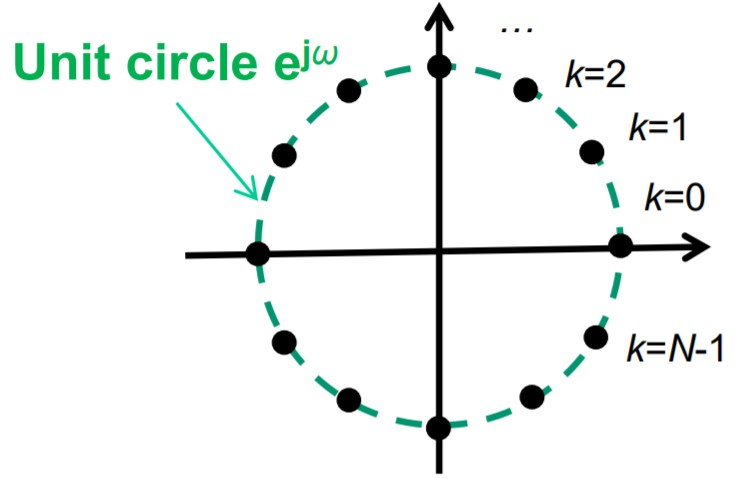
\includegraphics[width=5cm]{unit-circle}
		\caption{point on the Z plane on which the DFT is evaluated in order to have a \dft.} \label{fig:dft:unitcircle}
	\end{SCfigure}
	
	Intuitively, as can be deduced from figure \ref{fig:dft:unitcircle}, increasing the number of samples $N$ in the unit circle means decreasing the \textit{distance} between each angle $\omega_k$ and so for $N\rightarrow \infty$ the DFT computation converges to the DTFT.\\
	Note that the \dft is not an approximated version of the DTFT: in fact evaluating both function for the same angle $\omega_k$ will result in equal results, but the DFT is just a pure sampling of the DTFT in the frequency domain.
	
	\paragraph{Evaluation of the DFT} The \dft is so a better numerical formulation (in a sense that can be algorithmically implemented for automatic computation) that allows to estimate the spectra of a discrete-time signal. Even if the formulation in equation \ref{eq:dft:dft} can be automatized, the numerical cost complexity is quite high: better performance can be obtained by using the so called \de{Fast Fourier Transforms} \textbf{FFT} (better described lates), a set of complementary algorithms that aims at improving computational performance while still not impacting the final result.
	
	\paragraph{Inverse DFT} As for the Fourier transform, it's possible to define a \de{Inverse Discrete Fourier Transform}	 IDFT, an operator that allows to reconstruct a signal $x(n)$ from it's DFT $X(k)$:
	\begin{equation} \label{eq:dft:inversion}
		x(n) = \frac 1 N \sum_{n=0}^{N-1} X(k) e^{j\frac{2\pi}{N} kn } \hspace{2cm} \forall n = 0,\dots, N-1
	\end{equation}
	Such operation is the pure inversion of the DFT expression stated in equation \ref{eq:dft:dft}. We can in fact see that the spectrum can be computed as a linear combination of the the twiddle factors, in fact equation \ref{eq:dft:dft} can be expresses in a matrix form as
	\[ \underbrace{\begin{pmatrix}
		X(1) \\ X(2) \\ \vdots \\ X(N-1)
	\end{pmatrix}}_{\underline X} =  \underbrace{\begin{bmatrix}
		W_N^{1\cdot 1} & W_N^{1\cdot 2} & \dots & W_N^{1(N-1)} \\
		W_N^{2\cdot 1} & W_N^{2\cdot 2} & \dots & W_N^{2(N-1)} \\
		\vdots & \vdots & \ddots \\		
		W_N^{(N-1) 1} & W_N^{(N-1)\cdot 2} &  & W_N^{(N-1)(N-1)} \\
	\end{bmatrix}}_W \underbrace{\begin{pmatrix}
		x(1) \\ x(2) \\ \vdots \\ x(N-1)
	\end{pmatrix}}_{\underline x} \]
	Having the linear system $\underline X = W \underline x$, it's inversion $\underline x = W^{-1} \underline X$ is in fact the pure definition of the inverse \dft in equation \ref{eq:dft:inversion}.
	
	\subsection{Time aliasing}
		Given a discrete-time signal $x(n)$ with $L$ samples, meaning that
		\[ x(n)  \begin{cases}
			\neq 0 \qquad & n = 0,\dots, L-1 \\ = 0 & \textrm{otherwise}
		\end{cases} \]
		resulting  in a DTFT $X(e^{j\omega})$, the related \dft $X(k)$ can  be computed over a number of frequency discretization $N$ that's not necessary equal to $L$ (however this might sound the most common selection).
		
		Depending on the number of frequency discretization $N$ the application of the inverse \dft (equation \ref{eq:dft:inversion}) might lead to a reconstructed signal $\hat x(n)$ that's not necessary equal to the original sequence $x(n)$. By applying the definition in fact we have
		\begin{equation} \label{eq:dft:timealiasing}
		\begin{aligned}
			\hat x(n) & = \frac 1 L \sum_{k=0}^{L-1} \left( \sum_{m=0}^{N-1} x(m) e^{-j \frac{2\pi}{N}km} \right) e^{j\frac{2\pi}{L} kn} \\
			& = x(n) * \infsum r \delta(n-rN) = \infsum r x(n-rN)
		\end{aligned}
		\end{equation}
		From this result (obtained by computing the DTFT assuming $N\rightarrow \infty$ and after some algebraic manipulation) we can observe that
		\begin{itemize}
			\item if $N\geq L$ then the reconstructed signal $\hat x(n)$ is equal to the original signal $x(n)$;
			\item if $N < L$ then the reconstructed signal $\hat x(n)$ differs from the original $x(n)$.
		\end{itemize}
		
		The difference is due to the phenomena of the so called \de{\textit{time aliasing}} (shown in figure \ref{fig:dft:timealiasing}): from expression \ref{eq:dft:timealiasing} we can see that the IDFT computes a periodic signal with periodicity $N$ and so if $N < L$ then the last (and so the first) $L-N$ samples \textit{cyclically adds-up} by generating the phenomena of the time aliasing.		
		
		\begin{SCfigure}[2][bht]
			\centering 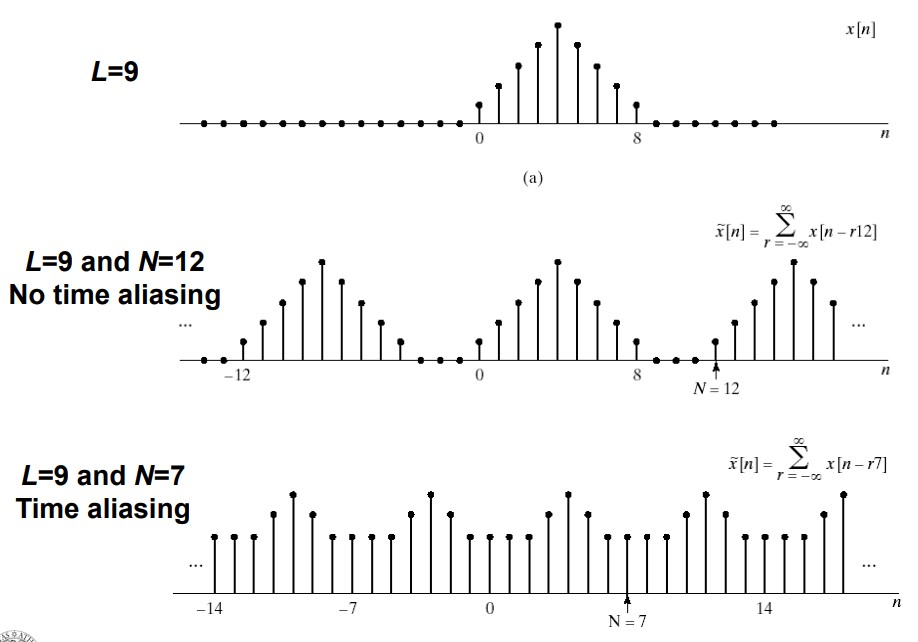
\includegraphics[width=8.5cm]{time-aliasing}
			\caption{ on top: original sequence $x(n)$ consisting of $L=9$ samples; below DFT+IDFT computed on $N = 12 (>L)$ and $N = 7(< L)$ samples; in the second case we can observe the phenomena of the time aliasing. } \label{fig:dft:timealiasing}
		\end{SCfigure}
		
		As was discussed at page \pageref{sec:conv:nyquist}, a sampling in the time domain can result in aliasing in frequency domain and so, dually, a sampling in the frequency domain results in time aliasing. The dual condition to the Nyquist frequency (eq. \ref{eq:conv:nyquist}, page \pageref{eq:conv:nyquist}) is so having 
		\begin{equation}
			N\geq L
		\end{equation}
	
	\subsection{Properties}
		
		The \dft is still a \textbf{linear operator}: given two discrete-time signals $x_1(n),x_2(n)$ having DFT's $X_1(k), X_2(k)$ then
		\begin{equation}
			ax_1(n) + b x_2(n) \qquad \mapsto \qquad aX_1(k) + bX_2(k) \hspace{2cm} \forall a,b \in \mathds R
		\end{equation}
		If this two sequences are characterized by different length $L_1,L_2$ (and as example we assume $L_2>L_1$), in order to apply such property is mandatory to perform the so called \de{\textit{zero padding}} that consist on adding $|L_1-L_2|$ zeros at the and of the shortest sequence (in this case the second) and then computing the DFT on $N = L_1 = L_2 + |L_1-L_2|$ (or on a higher \textit{sampling in the frequency domain}).
		
		\paragraph{Circular shifting} Given a sequence $x(n)$ of $L$ samples with associated \dft $X(k)$, then given an integer time shift of $m\in \mathds Z$ samples determines
		\begin{equation}
			\tilde x(n-m) \quad \textrm{with } n =0,\dots, N-1 \hspace{1.2cm} \mapsto \qquad X(k) e^{-j\frac{2\pi k}{L}m}
		\end{equation} 
		where $\tilde x(n)$ is the \textit{infinite repetition} of the signal $x(n)$ obtained by it's iterative concatenation.
		
		\paragraph{Symmetries} As for the Fourier transform, if the discrete-time signal $x(n)$ is real evaluated, then the DFT (with a frequency sampling of $N$ samples) of such signal presents an even symmetry on the real axis, and in particular we obtain
		\begin{equation}
			\Re{X(k)} = \Re{X(N-k)} \hspace{2cm} \Im{X(k)} = - \Im{X(N-k)}
		\end{equation}
		
		\paragraph{Convolution and circular convolution} Given two discrete-time signals $x_1(n),x_2(n)$ having each length $L,P$ and DFT $X_1(k),X_2(k)$, then the \textit{linear} convolution property still holds:
		\begin{equation}
			x_3(n) = x_1(n) * x_2(n) \qquad \mapsto \qquad X_3(k) = X_1(k) X_2(k)
		\end{equation}
		With this definition, by computing the inverse \dft we retrieve a periodic signal $ \tilde x_3(n) = \tilde x_1(n) * x_2(n) = x_1(n) * \tilde x_2(n)$ that differs from the expected $x_3(n)$.\\
		Considering instead a convolution performed over $N$ samples, then such signal is referred as \de{circular convolution} defined as
		\begin{equation}
			x_1(n) \circconv N x_2(n) := \sum_{m=0}^{N-1} x_1(m) \tilde x_2(n-m)
		\end{equation}
		In order to perform a proper \dft that holds $x_1(n)*x_2(n) = x_1(n) \circconv N x_2(n)$ we must ensure that the DFT is computed over a set of frequency sample $N \geq L+ P - 1$; if this condition isn't met, then linear and circular convolution results are different.
		
		\paragraph{Impulse response} As was described in section \ref{sec:conv:impulseresponse} (page \pageref{sec:conv:impulseresponse}), we denote as $h(n)$ the impulse response of a discrete-time system and in the case it present a finite impulse response (FIR system) with $P$ non-zero samples, so such that
		\[ h(n) \neq 0 \qquad \textrm{for } n = 0,\dots, P-1 \]
		Assuming to have an input $x(n)$ made of $L$ non-zero samples, then the output $y(n)$ of the system can be described by the linear convolution (that has a maximum of $L+P-1$ non-zero samples):
		\[ y(n) = x(n) * h(n) \neq 0 \qquad \textrm{for } n=0,1,\dots, L+P-2 \]
		
		Solving this problem in the frequency domain using the \dtft, known the transforms $X(e^{j\omega}), H(e^{j\omega})$  we obtain the frequency response as multiplication of this two spectrum:
		\[ Y(e^{j\omega}) = X(e^{j\omega}) H(e^{j\omega}) \qquad \xrightarrow{\F^{-1}} \qquad y(n) \]
		
		Knowing that the analytical solution is not practical from a numerical point of view, we have to use the \dft that can algorithmically implemented. Known the discrete transforms $X(k),H(k)$ made by $L,P$ samples each, then in order to perform a proper convolution operation we have to set both initial signals $x(n),h(n)$ to a length $N=L+P-1$ (by so performing a zero-padding of $P-1$ samples on $x(n)$ and of $L-1$ samples on $h(n)$): after this operation we are sure that the DFT product $X(n)H(n)$ has a number of samples $N = L+P \geq L+P-1$ that allows to have a proper linear convolution without time aliasing.		
		
\section{Fast Fourier transforms}
	
	\de{Fast Fourier Transforms} \textbf{FFT}s are a class of algorithms used to compute \textit{in a faster way} (by decreasing the numerical computational complexity) of the \dft by using some \textit{mathematical tricks} that are gonna shown later.
	
	\paragraph{Computational cost} Considering the formal definition of the DFT state on page \pageref{eq:dft:dft} (equation \ref{eq:dft:dft}) we can see that the computation of a spectrum with $N$ samples in the frequency domain involves $N-1$ complex additions and $N$ complex multiplications for each spectral sample and so the overall cost is
	\[ N(N-1) \text{ complex additions} \qquad + \qquad N^2 \text{ complex multiplications} \]
	Each complex multiplication relies on 4 real multiplications and 2 real addition while the complex addition is made by two real summation: this means that to compute a DFT/IDFT $4N^2$ real multiplication and $N(4N-2)$ real additions are required, with an overall algorithm complexity of 
	\[ \mathcal O(N^2 ) \]
	
	This means that the overall computational time needed to compute a DFT/IDFT grows quadratically with the number of samples required: such relation is \textit{far-from-good} considering that in real world application DFTs must be applied on signal with a arbitrary large size (tens of thousands or more). The best Fast Fourier transform algorithms can reduce the computational complexity to the best numerical complexity order
	\[ \mathcal O\big( N \log_2N \big) \]
	Usually this algorithms in order to  be as effective as possible required a value of $N$ that's a power of two, so such that the frequency samples length can be expressed as
	\begin{equation} \label{eq:dft:pow2}
		 N = 2^\nu \hspace{2cm} \textrm{with } \nu \in \mathds N
	\end{equation}
	
	\subsection{Decimation in time}
		
		\de{Decimation in time} is a \fft algorithm whose main idea is to recursively bisect the original DFT into transforms with half size and then \textit{cleverly} recompose them together. This algorithm, in order to work, requires a number $N$ of samples that's a power of 2 (equation \ref{eq:dft:pow2}).
		
		Considering the discrete-time sequence $x(n) \neq 0$ for $n=0,\dots, N-1$ (with $N=2^\nu$), then such signal can be bisected in two sequences of length $N/2$ (that's still an integer equal to $2^{\nu-1}$) determined by the values in odds and even positions:
		\begin{equation}
			\underbrace{x(0),x(2),\dots, x(N-2)}_{x_e(r) = x(2r)} \hspace{2cm} \underbrace{x(1),x(3),\dots, x(N-1)}_{x_o(r) = x(2r+1)} 
		\end{equation}
		with $r = 1,\dots, \frac N2-1$. Considering the formal definition of the \dft (equation \ref{eq:dft:dft}, page \pageref{eq:dft:dft}) we can compute \textit{bisect} the definition of the transform considering the even and odd sequence, in fact:
		\begin{equation} \label{eq:dft:temp1}
			X(k) = \sum_{n=0}^{N-1} x(n) W_{N}^{kn} = \sum_{r=0}^{\frac N2-1} x(2r) W_N^{2rk} + \sum_{r=0}^{\frac N2-1} x(2r+1) W_N^{(2r + 1)k}
		\end{equation}
		From the definition of the twiddle factor $W_N = e^{-j\frac{2\pi}{N}}$ can can observe that $W_N^2 = W_{N/2}$, in fact
		\begin{equation}
			W_N^2 = e^{-j\frac{2\pi}{N}2} = e^{-j\frac{2\pi}{N/2}} = W_{N/2}
		\end{equation}
		Observing also that $W_N^{(2r+1)k}$ can be regarded as $W_N^k W_N^{2rk}$ using the power's properties, then equation \ref{eq:dft:temp1} can be rewritten as a combination of the spectrum of the even and odd sub-samples in the form
		\begin{equation}
		\begin{aligned}
			X(k) & = \sum_{r=0}^{\frac N2-1} x_e(r) W_{N/2}^{rk} + W_N^k\sum_{r=0}^{\frac N2-1} x_o(r) W_{N/2}^{rk} \\
			& = X_e(n) + W_N^k X_o(k)
		\end{aligned}
		\end{equation}
		
		\paragraph{Computational cost} Exploiting this idea we can reduce the numerical complexity. We can see in fact that the number of twiddle factor that must be computed is halved (from $N$ of the original case to $N/2$, in fact the twiddle factors for both even and off spectrum are equals). Also considering that halving of the DFT computation size reduces by $1/4$ the computational cost (considering the DFT complexity of $\mathcal O(N^2)$), then
		\[ \mathcal O\Big( X_e(k) + X_o(k) \Big) \propto \frac{N^2}{4} + \frac{N^2}{4} + N < N^2 \qquad \textrm{for } N > 2  \]
		By applying recursively the concept of bisecting the spectrum computation (in fact both sequences $x_e(n),x_o(n)$ can still be subdivided in other even/odds sequences), the asymptotic computational complexity drops from $\mathcal O(N^2)$ to
		\[ \mathcal O\big(N\log_2N\big) \]
		
		\paragraph{Graph representation} Continuing bisecting the original sequence $x(n)$ (this is possible by the assumption of having $N=2^\nu$) we reach the end of recursion when the \textit{sub-obtained} sequence has a base length of 2: from this point on is in fact possible to reconstruct the spectrum of the original signal.	
		
		\begin{SCfigure}[2][bht]
			\centering 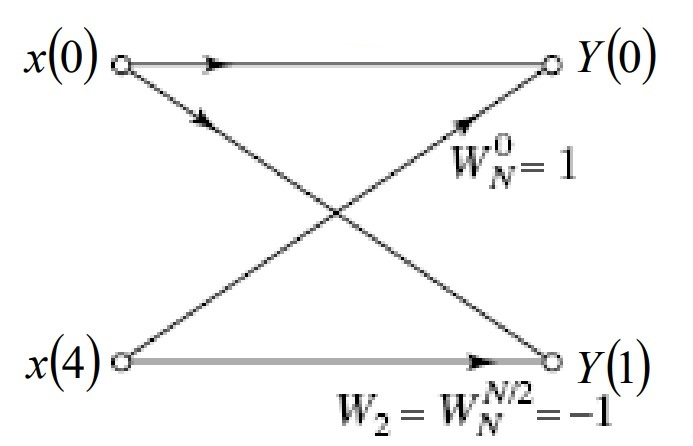
\includegraphics[width=4cm]{fft-dec-graph-bin}
			\caption{graph representation of the \fft using the decimation in time algorithm computed on 2 points starting from a signal of length $N=8$.} \label{fig:dft:fftsing}
		\end{SCfigure}
		
		Reached this point, as shown in figure \ref{fig:dft:fftsing}, we can see that we have only two twiddle factors (that in this case are all real-evaluated) $W_N^0 = 1$ and $W_2 = W_N^{N/2} - 1$ that allows to compute the 2 spectral component of the bisected signal as
		\[ X(0) = x(0) + x(1) \hspace{2cm} X(1) = x(0)- x(1) \]
		
		\begin{figure}[b!t]
			\centering
			\begin{subfigure}{0.48\linewidth}
				\centering 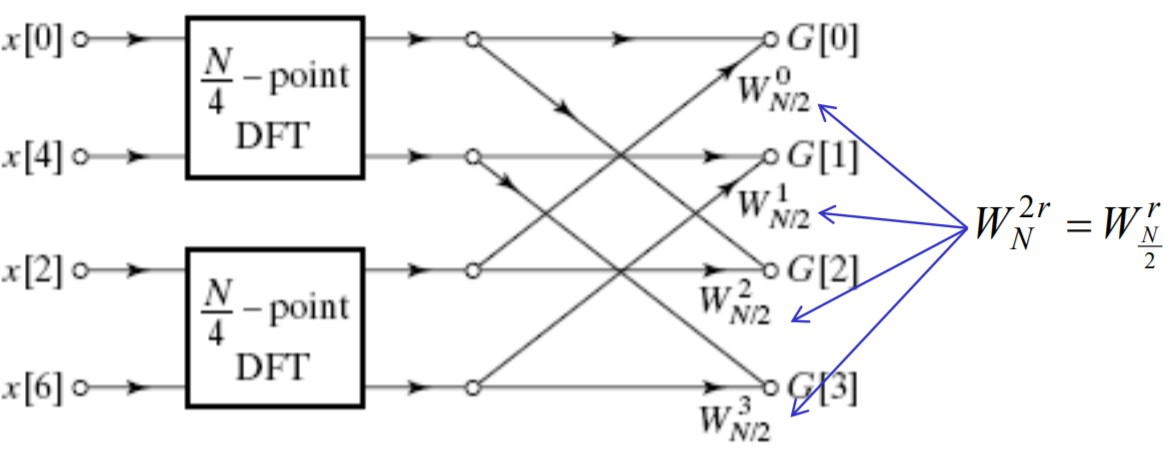
\includegraphics[width=0.9\linewidth]{fft-dec-graph-sec} \caption{}
			\end{subfigure}
			\begin{subfigure}{0.48\linewidth}
				\centering 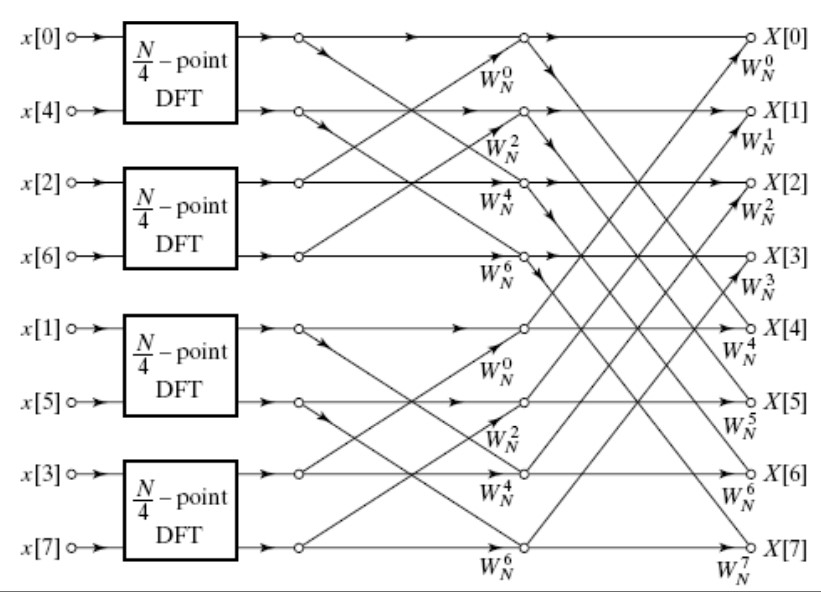
\includegraphics[width=\linewidth]{fft-dec-graph-comp} \caption{}
			\end{subfigure}
			\caption{second (a) and third (last) (b) step of the computation of the DFT on a signal having $N=8$ samples using the decimation in time FFT algorithm.} \label{fig:dft:fftcomp}
		\end{figure}
		
		With the smallest spectra computed, the spectrum re-combination can take place as shown in figure \ref{fig:dft:fftcomp}; considering the second stage of the decimation in time algorithm (fig. \ref{fig:dft:fftcomp}.a) the 4 spectral components are computed as linear combination of 2 elements retrieved one each from the 2 sub-computed spectra of the first stage. The twiddle factors are computed considering the properties $W_N^{2r} = W^r_{N/2}$. The third stage spectral components are so a linear combination of 2 elements from the previous  recursive definition and the recursion keeps going on until reaching the full spectrum of the signal.	 	
		
		\paragraph{Modularity of the decimation in time algorithm} A point of force of the decimation in time FFT algorithm is it's recursion and modularity mainly determined by the \textit{butterfly structure} (name took by the butterfly-look-like graph in figure \ref{fig:dft:fftsing}) and in particular we can observe that
		\begin{itemize}
			\item the algorithm cleverly uses the memory: results of the iterative-recursive stages can be overwritten in the same memory address. The out-of-order samples (as seen on the left side in figure \ref{fig:dft:fftcomp}.b) can be in fact accessed using reversed-bit mode available in all digital signal processing processors:
			\begin{center}
			\begin{tabular}{ M{1cm} M{1.3cm} M{1.3cm} M{1cm} }
				& index & address & \\ \hline
				$x(0)$ & 000 & 000 & $X(0)$ \\ 
				$x(4)$ & 100 & 001 & $X(1)$ \\
				$x(2)$ & 010 & 010 & $X(2)$ \\
				$x(6)$ & 110 & 011 & $X(3)$ \\
				$x(1)$ & 001 & 100 & $X(4)$ \\
				$x(5)$ & 101 & 101 & $X(5)$ \\
				$x(3)$ & 011 & 110 & $X(6)$ \\
				$x(7)$ & 111 & 111 & $X(7)$
			\end{tabular}
			\end{center}
			
			\item the butterfly computation can extended not just to the first stage, but for any $m$-th stage. Considering in fact the spectral components coming from the $X_{m-1}(p),X_{m-1}(q)$ the $m-1$-th stage, the new computed spectral components of the $m$-th stage are stored in the same spot and it happens that
			\begin{equation}
				X_m(p) = X_{m-1}(p) + W_N^r X_{m-1}(q) \hspace{0.5cm} X_m(p) = X_{m-1}(p) - W_N^r X_{m-1}(q)
			\end{equation}
			where the change of sign on the twiddle factor is obtained considering that
			\[ W_N^{r+ \frac N2} = W_N^r W_N^{N/2} = - W_N^r \]
			where $t$ is the coefficient depending on the stage of calculation.
		\end{itemize}
	
	\subsection{Decimation in frequency}
		
		From every FFT algorithm a dual one can be generated in order to compute the inverse \fft; the \de{decimation in frequency} is in fact the dual \textit{representation} of the decimation in time algorithm that allows to reconstruct a signal in the time domain if it's discrete Fourier transform has a number of sample $N$ that's a power of 2 (so in the form $N=2^\nu$).
		
		\begin{figure}[b!]
			\centering 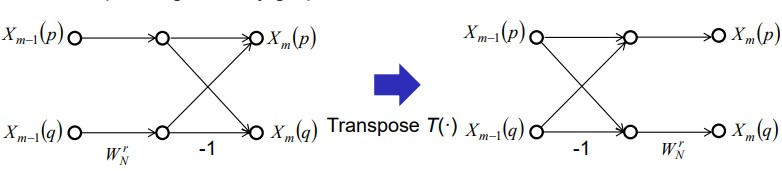
\includegraphics[width=10cm]{fft-dec-stage}
			\caption{graph representation (right) of the decimation in frequency algorithm butterfly as the transposition of the decimation in time one (left).} \label{fig:dft:decfreq}
		\end{figure}
	
		The working principle is the same: the spectrum $X(k)$ is recursively bisected in it's even $X_e(k) = X(2k)$ and odd $X_o(k) = X(2k+1)$ \textit{part} until reaching the recursion limit of a sequence of length $2$. From this point on the butterfly graph to implement, as shown in figure \ref{fig:dft:decfreq} is the transposed one of the decimation in time.
		
		\paragraph{Graph transposition} Given a graph $\delta(N,\varepsilon)$ of $N$ edges $\varepsilon$, then it's transition $\delta^t(N,\varepsilon')$ is obtained by reversing the direction of the edges: the input so becomes the output and vice-versa. The weight of the edges stays unaltered.		
			
\section{Spectral estimation}
	
	The \de{spectral  estimation} is the analysis of signals using techniques in the frequency domain in order to provide informations regarding the behaviour of the system. Real signals are usually stochastic (and not deterministic) and so computing the proper spectra isn't in general a easy problem. Depending on the type of process we are analysing we can classify the signals and so the techniques that can be used as shown in table \ref{tab:dtf:specestim}
	
	
	\begin{table}[bht]
	\centering
	\tabrule
	\caption{spectral estimation classifications.} \label{tab:dtf:specestim} \vspace{2mm}
	
	\begin{tabular}{ M{0.22\linewidth} M{0.22\linewidth} | M{0.22\linewidth} M{0.22\linewidth} }
		\multicolumn{4}{c}{\textbf{Spectral Estimation}} \\  \\ 
		\multicolumn{2}{c|}{deterministic signals (finite energy)} & \multicolumn{2}{c}{random processes (finite power)} \\ &&&\\
		stationary & non-stationary & stationary & non-stationary \\
		$\Downarrow$ & $\Downarrow$ & $\Downarrow$ & $\Downarrow$ \\
		Fourier transform & short-time Fourier transform & power spectral density (PSD) & PSD as a function of time \\
		$\Downarrow$ & $\Downarrow$ & $\Downarrow$ & $\Downarrow$ \\
		DTF/FFT & Discrete STFT & average periodogram and other estimators & spectrogram, short-time periodogram		
	\end{tabular}\vspace{3mm}	
	\tabrule
	\end{table}
	
	If a system is stationary the quality of the estimation doesn't depend on the time on which we perform the estimation itself, while this isn't true for non-stationary signals on we we want to track all the changes of the signal over time.
	
	\subsection{Stationary deterministic signal}
		
		Focusing on the case of a continuous-time \textbf{stationary deterministic signal} $x_c(t)$, the ideal way to perform a spectral estimation is by \textit{simply} computing its \ctft in order to determine the spectrum $X_c(\Omega)$. This is easier said than done, and in real application such operation is not feasible and to do so we necessarily need to discretize the time axis with a certain sampling period $T_s$  and estimate a discrete spectrum $\hat X_c(\Omega) \approx X_c(\Omega)$.
	
		\begin{figure}[bht]
			\centering
			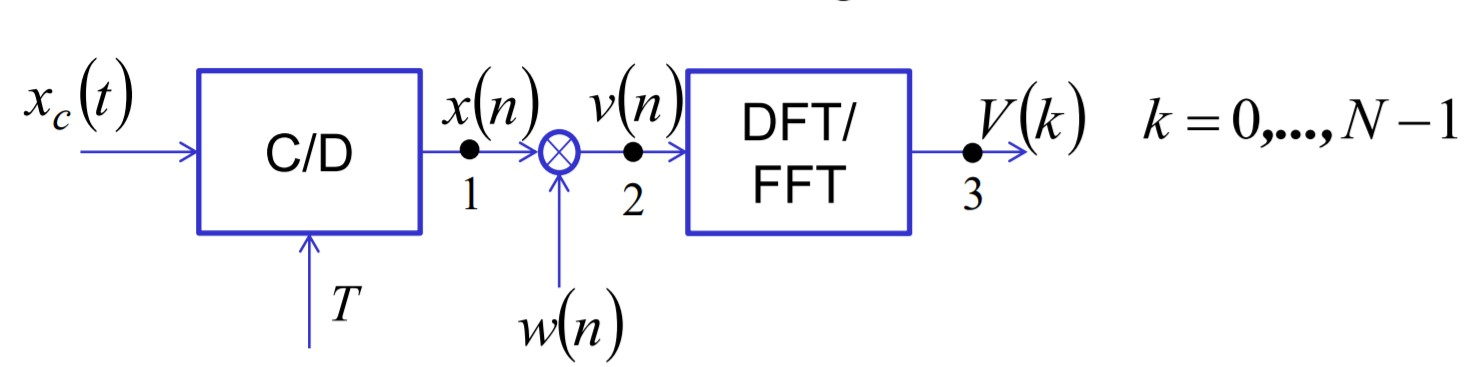
\includegraphics[width=8cm]{deterministic-estimation}
			\caption{steps that has to be performed in order to estimate a stationary deterministic signal.}
			\label{fig:dft:statdetsignalestimation}
		\end{figure}
		
		As it can be seen in figure \ref{fig:dft:statdetsignalestimation}, to perform the estimation we firstly discretize the signal into a discrete-time sequence $x(n)$, determining a change of the original spectrum $X_c(\Omega)$ with the addition of aliases in the transform (as it was discussed in section \ref{sec:conv:timeconversion}, page \pageref{sec:conv:timeconversion}):
		\begin{equation}
			X\big(e^{j\omega}\big) = \frac 1 {T_s} \infsum k X_c\left( \frac \omega{T_s} + \frac{2\pi k}{T_s} \right)
		\end{equation}
		
		After that we have to consider that not physically/computationally feasible to determine the \dtft of a signal with infinite length (it's impossible to store such quantity of data and compute the DFT on it), and so we have to rely on just a \textit{segment} of the whole data. Considering a rectangular \textbf{window} of $L$ samples defined as
		\[ w(n) = \begin{cases}
			1 \qquad & n = 0,\dots, L-1 \\ 0 &\textrm{otherwise}
		\end{cases} \]
		then the signal $v(n)$ that can be processed is the one obtained by multiplying such window with the discretized sequence $x(n)$:
		\[ v(n) = x(n)w(n) \]
		This means that the spectrum that we can estimate is also influenced by the convolution  of the two signals considering the related property and so
		\begin{equation}
			V\big(e^{j\omega}\big) = X\big(e^{j\omega}\big) * W\big(e^{j\omega}\big) = \frac 1{2\pi} \int_{-\pi}^\pi X\big(e^{j\theta}\big) W\big(e^{k(\omega-\theta)}\big)\, d\theta \neq X\big(e^{j\omega}\big)
		\end{equation}
		\begin{note}
			in general other windowing function $w(n)$ can be used (as it's going to be explained later) in order to differently affect the spectral estimation.
		\end{note}
	
		From a practical point of view the only way to estimate the spectrum is by computing the \dft $V(k)$, a \textit{sampled} version of the \textit{continuous} spectrum $V(e^{j\omega})$ in the frequency domain. As a rule of thumb the discretization value $N$ for the 	DFT computation should always be grater (or equal) to the length $L$ of the window (in order not to have the time aliasing problem while returning in the time domain after signal processing).	
		
		\subsubsection{Effect of windowing on the spectral estimation of a cosine wave} Considering the continuous-time sinusoidal signal $x_c(t) = A \cos(\Omega_0 t +\theta_0)$, as was previously seen, it's spectrum (shown in figure \ref{fig:dft:cosinespectrum}) consists of two dirac pulses at frequencies $\pm \Omega_0$ with a complex amplitude of $\frac A 2 e^{-j\theta_0}$.
		
		\begin{SCfigure}[2][bht]
			\centering 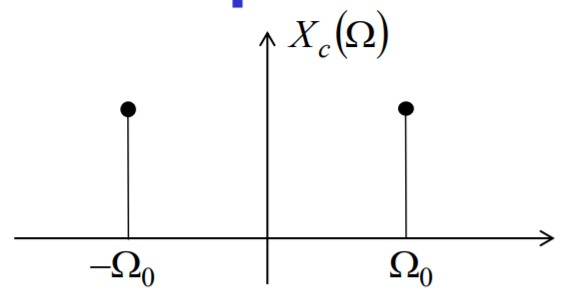
\includegraphics[width=5cm]{sin-spect}
			\caption{magnitude spectrum of the signal $A \cos(\Omega_0t+\theta_0)$.}
			\label{fig:dft:cosinespectrum}
		\end{SCfigure}
		
		Considering it's discretized version $x(n) = A\cos(\omega_0n + \theta_0)$ (where $\omega_0 = \Omega_0 T_s$) then the windows signal $v(n)$ on which the DFT can be computed is
		\begin{align*}
			v(n) & = x(n) w(n) = A w(n)\, \cos(\omega_0n + \theta_0) \\
			& = \frac A 2 w(n) e^{j\theta_0} e^{j\omega_0n} + \frac A 2 w(n) e^{-j\theta_0} e^{-j\omega_0n} 
		\end{align*}
		Knowing the \dtft of the signal $e^{j\omega_0n}$ as $\delta(\omega-\omega_0)$, then the spectrum $V(e^{j\omega})$ of the sequence can be regarded
		\begin{equation} \label{eq:dft:windowedcosine}
			V \big(e^{j\omega}\big) = \frac A 2 e^{j\theta_0} W\big( e^{j(\omega-\omega_0)}\big) +  \frac A 2 e^{-j\theta_0} W\big( e^{j(-\omega+ \omega_0)}\big)
		\end{equation}
		
		To determine the \textit{distortion} due to the window it's necessary to compute it's spectrum; considering in fact the sequence $w(n) e^{-j\omega n}$ the DTFT is computed as
		\begin{align*}
			W\big(e^{j\omega}\big) & = \infsum n w(n) e^{-j\omega n} = \sum_{n=0}^{L-1} e^{-j\omega n} = \frac{1-e^{-j\omega L}}{1-e^{-j\omega}} \\
			& = e^{-j\omega \frac{L-1}{2}} \frac{\sin\left(\frac{\omega L}{2}\right)}{\sin\left(\frac \omega 2\right)}
		\end{align*}
		\begin{note}
			the \dtft  of the window has been computed the convergent geometrical sequence summation described in the note at page \pageref{sec:four:geometricalprogression}.
		\end{note}
		The term $\frac{\sin(\omega L/2)}{\sin(\omega/2)}$ is known as the \de{Dirichlet-Kernel} function characterized by being equal to $L$ for $\omega_0$ and being null for each multiple of the frequency $\frac{2\pi}{L}$; in figure \ref{fig:dft:dirichkernel} it's spectrum has been represented.
		
		\begin{figure}[bht]
			\begin{subfigure}{0.48\linewidth}
				\centering 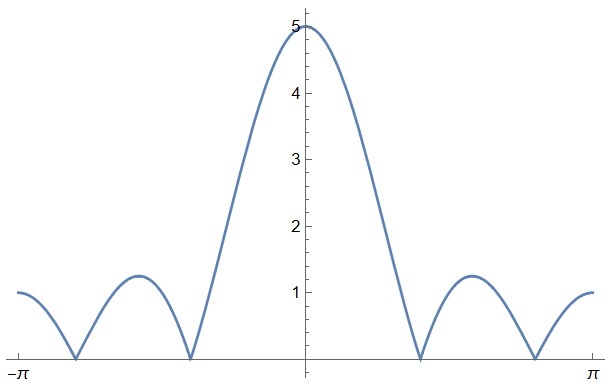
\includegraphics[width=5cm]{dirich-kernel} \caption{}
			\end{subfigure}
			\begin{subfigure}{0.48\linewidth}
				\centering 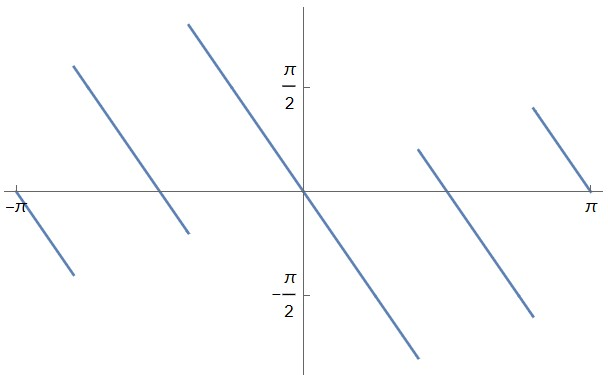
\includegraphics[width=5cm]{dirich-kernel-phase} \caption{}
			\end{subfigure}
			\caption{magnitude (a) and phase (b) of the Dirichlet-Kernel function.}
			\label{fig:dft:dirichkernel}
		\end{figure}
		
		\noindent For this Dirichlet-Kernel function we refer the \textit{central peek} as the \textbf{main-lobe} (with a peak equals to $L$) while the other \textit{bell-shaped} segments are referred as \textbf{side-lobes}; this function is characterized by the main-lobe width $\Delta_w = 4\pi/L$ parameter; we can also observed that the spectrum (figure \ref{fig:dft:dirichkernel}.b) has a so called \textbf{\textit{generalized linear phase}}. \vspace{3mm}
		
		With the definition of the Dirichlet-Kernel function, the spectrum of the windowed cosine function (equation \ref{eq:dft:windowedcosine}) isn't just made of two pulses at frequencies $\pm \omega_0$, but it's composed by two Dirichlet-Kernel functions with main-lobes center at frequencies $\pm\omega_0$ (on which the pulses were expected), as shown in figure \ref{fig:dft:spectrdistorted}.
		
		\begin{SCfigure}[2][bht]
			\centering 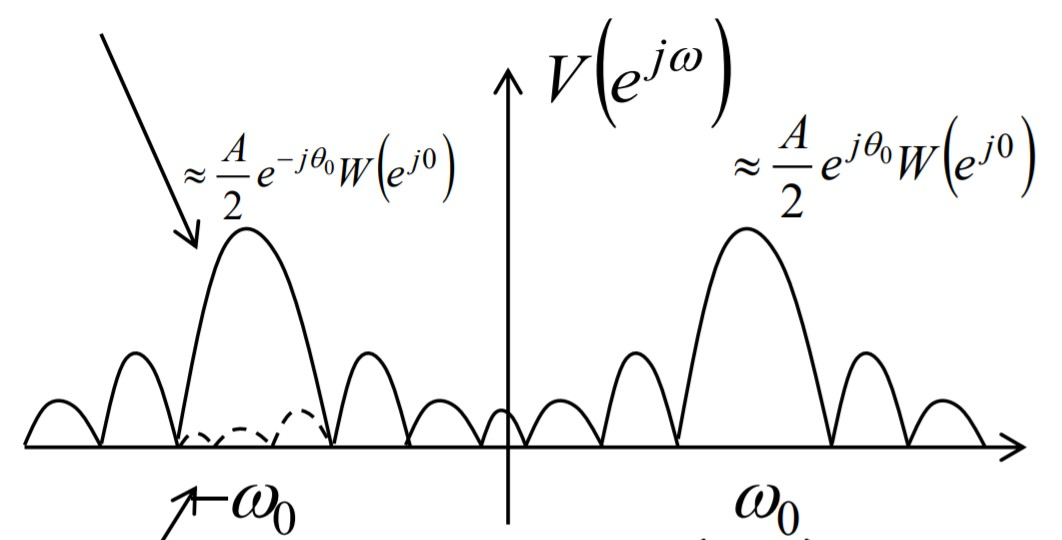
\includegraphics[width=6cm]{sin-modified}
			\caption{spectrum of the signal  $v(n)= x(n)w(n)$ that's distorted due to the windowing.}
			\label{fig:dft:spectrdistorted}
		\end{SCfigure}  
	
		To reduce the effect ot the lobes of the Dirichlet-Kernel function it's necessary to reduce the main-lobe width $\Delta_w$ by increasing the number of samples $L$ collected by the window (for $L\rightarrow \infty$ the Dirichlet-Kernel tends to the Kronecker delta). Practically this operation of increasing the length of samples $L$ can be pushed up to a certain limit (time/numerical complexity) and the problem that we get from this limitation are
		\begin{itemize}
			\item the \textbf{spectral leakage}: considering the case shown, the theoretical energy of the sinusoidal signal is concentrated at the frequencies $\pm\omega_0$, however with the addition of the windowing there's a sort of \textit{leak} that spreads out the energy all over the frequency axis;
			
			\item the \textbf{spectral infiltration}, related to the leakage, refers to the fact that the principal side-lobes (the ones next to the main-lobe) might interfere with main-lobes of other function's transforms. It can be noted that the ratio between main and principal side-lobe is constant and weakly depends on the number of samples $L$;
			
			\item the \textbf{finite spectral resolution}: considering a signal that's a sum of cosine function of the form $x_c(t) = A_1 \sin(\Omega_1t + \theta_1) + A_2 \sin(\Omega_2t+\theta_2)$, then the theoretical DTFT consists of dirac pulses centred at the frequencies $\pm \omega_1,\pm \omega_2$, however the estimated spectrum due to the window is
			\[ V \big(e^{j\omega}\big) = \sum_i \frac{A_i}{2} e^{\pm j\theta_i} W\Big( e^{j(\omega \mp \omega_i)} \Big) \]
			Depending on the length $L$ of the window, if the frequencies $\omega_1,\omega_2$ are \textit{sufficiently close together} the main-lobes associated related to the windows of the cosine might interfere (as shown in figure \ref{fig:dft:spectralresolution}). In order to avoid such problem we have to ensure that
			\[ |\omega_1-\omega_2| > \frac{\Delta_w}{2} \]
			
		\end{itemize}
	
		\begin{SCfigure}[2][bht]
			\centering 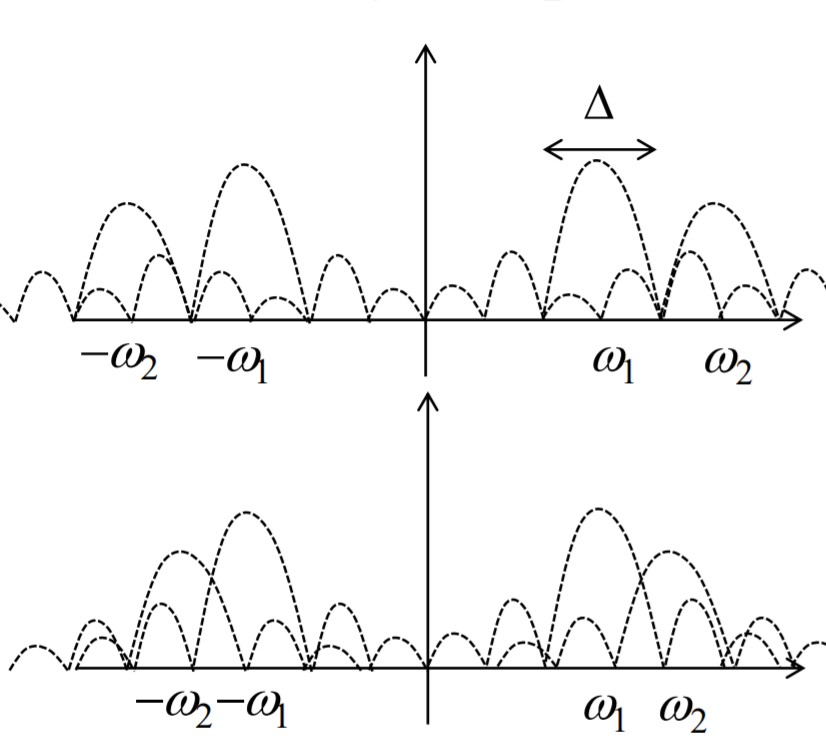
\includegraphics[width=6cm]{spectral-resolution}
			\caption{estimated spectrum of a signal $ A_1 \sin(\Omega_1t + \theta_1) + A_2 \sin(\Omega_2t + \theta_2)$ where the difference $\omega_1-\omega_2$ is "big" and so the spectral leakage can be neglected (upper) and the case on which the frequencies are "sufficiently close" (lower) considering the problem of the spectral resolution.} \label{fig:dft:spectralresolution}
		\end{SCfigure}
	
		\subsubsection{Windowing functions}
		In general other windowing function $w(n)$ different from the rectangular one can be constructed in order to minimize the errors/problem related to the spectral estimation. Performances can be improved by increasing, as example, the ratio between the main-lobe and the principal side-lobes or lowering the main-lobe width $\Delta_w$ for the same window length $L$. In figure \ref{fig:dft:windowfunctions} a set of windowing functions have been presented in both the time domain and frequency magnitude response.
		
		\begin{figure}[bht]
			\centering 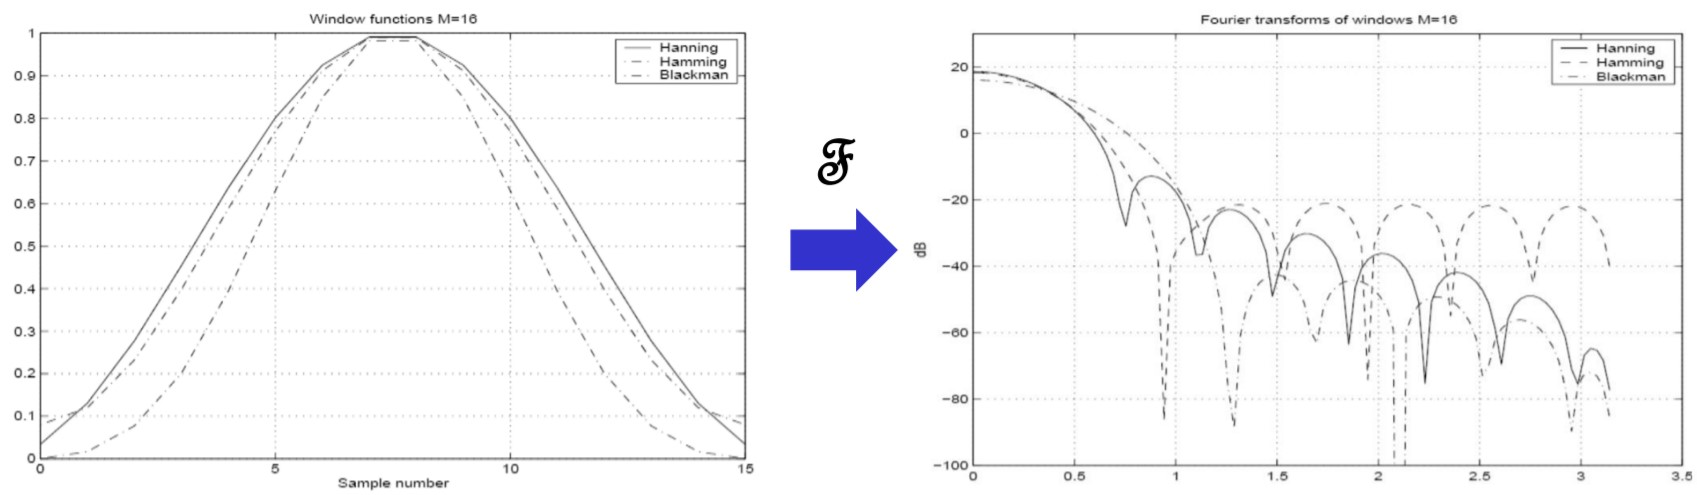
\includegraphics[width=\linewidth]{windowfunctions}
			\caption{windowing functions and relative magnitude of the Fourier transforms.}
			\label{fig:dft:windowfunctions}
		\end{figure}
		
		Table \ref{tab:dft:windowfunctions} resumes the main characteristics of some window functions; in particular we can see that (for a fixed length $L$ of the window) the side/main-lobe ratio is inversely proportional to the main-lobe width (lower $\Delta_w$ positively affects the resolution with the drawback of a higher \textit{side-lobe infiltration} impact).
		
		\begin{table}[bt] \centering \tabrule
			\caption{list of possible windows with relative side to main-lobe radio (in decibels) and main-lobe width (depending on number of windowed samples $L$).}
			\label{tab:dft:windowfunctions}
			\begin{tabular}{M{0.25\linewidth} M {0.25\linewidth} M{0.25\linewidth} }
				window & side/main-lobe ratio & main-lobe width $\Delta_w$\\ \hline
				rectangular & $-13db$ & $4\pi/L$ \\
				Bartlett (triangular) & $-25db$ & $8\pi/L$ \\
				Hanning & $-31db$ & $8\pi/L$ \\
				Hamming & $-41db$ & $8\pi/L$ \\
				Blackman & $-57db$ & $12\pi/L$ \\
			\end{tabular} \tabrule
		\end{table}
	
		\paragraph{Cosine class windows} The \textbf{Hanning}, \textbf{Hamming} and \textbf{Blackman} functions belongs to the \de{cosine class windows} of order $K$ whose general formulation is
		\begin{equation} \label{eq:dft:cosinewindows}
			w(n) = \sum_{k=0}^K a_k \cos \left(\frac{2\pi k}{L}n\right)\, dk
		\end{equation}
		Hanning and Hamming are both first order cosine windows with respective coefficients $a_0 = \frac 1 2,a_1 = - \frac 1 2$ and $a_0 = 0.54,a_1 = -0.46$; the Blackman filter is instead a second order filter. The general formulation of the main-lobe width of cosine-class function is
		\begin{equation}
			\Delta_w = \frac{4\pi}{L} \big(K+1\big)
		\end{equation}
		
		Respect to table \ref{tab:dft:windowfunctions}, fixed the length $L$ of the window going from the rectangular to the Blackman window worsen the resolution while improving on the spectral leakage side (and so is always a tradeoff between this two characteristic: resolution vs spectral leakage).
		
		\subsubsection{Frequency discretization}
		Until now we referred to the \dtft $V\big(e^{j\omega}\big)$ of the sampled signals, however in practise the tool that we can use is the \dft (FFT algorithms) computing the discretized spectrum $V(k)$. Considering, as reference, the case of the co-sinusoidal function whose transform is described in equation \ref{eq:dft:windowedcosine}, the choice of the number $N$ of frequency discretization heavily affects the read of the spectrum itself; for that reason 3 particular scenarios (graphed in figure \ref{fig:dft:samplingvariation}) can happen:
		\begin{enumerate}
			\item \textbf{coherent sampling} happens when one of the spectral sample lies exactly at the frequency $\omega_0$ while the other samples coincides with the zeros of the window spectrum; in this case the spectrum is clearly read by the DFT and the effect of leakage is negligible. This kind of operation can be performed in general only for periodic signals (on which it's relatively \textit{easy} to determine the number of samples $N$ that minimises the leakage) due to the fact that the ideal spectrum is composed by a sequence of pulses;
			
			\item \textbf{non-coherent sampling} happens when the peak lies between the two spectral samples; in this case there's \textit{a lot} of uncertainty in both magnitude and phase response of the expected frequency peak due to the evident effect of spectral leakage;
			
			\item increasing the number of samples in a non-coherent sampling improves estimation by having a higher frequency resolution (that doesn't mean having a higher quality estimation) but that doesn't get rid of the spectral leakage that's still present.			 
		\end{enumerate}
		
		\begin{figure}[bt]
			\begin{subfigure}{0.32\linewidth}
				\centering 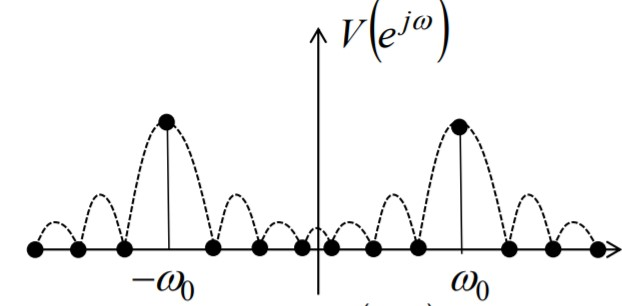
\includegraphics[width=0.9\linewidth]{sampling-1} \caption{}
			\end{subfigure}
			\begin{subfigure}{0.32\linewidth}
				\centering 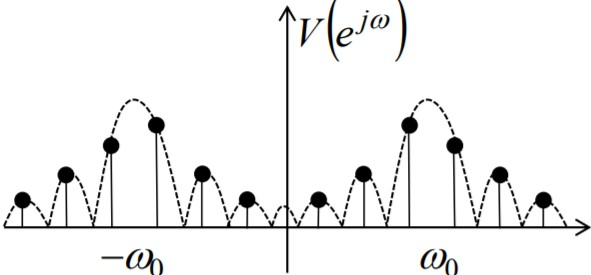
\includegraphics[width=0.9\linewidth]{sampling-2} \caption{}
			\end{subfigure}
			\begin{subfigure}{0.32\linewidth}
				\centering 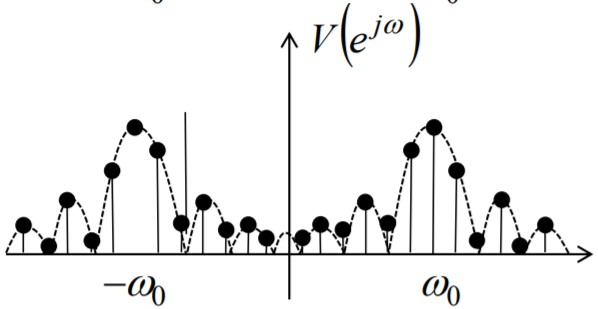
\includegraphics[width=0.9\linewidth]{sampling-3} \caption{}
			\end{subfigure}
			\caption{coherent sampling (a), non-coherent sampling (b) and non-coherent sampling with higher number of samples $N$ (c).}
			\label{fig:dft:samplingvariation}
		\end{figure}
				
	\subsection{Non-stationary deterministic signal: short time Fourier transform}
		
		A simple example of \textbf{non-stationary deterministic signal} is a sinusoidal function with frequency changing over time:
		\[ x_c(t) = \cos\big(\Omega(t)\,t\big)  \hspace{2cm} \text{where } \Omega(t) = \Omega_0 t \]
		Evaluating this signal at a time $t_0$ we expect, as spectral response, a Dirac pulse centred at the frequency $\pm \Omega(t_0)$, but if we evaluate the same signal at another time $t_1\neq 0$ such pulses are shifted to different frequencies $\Omega(t_1)$.
		
		In practise the tools that we can use to perform the spectral estimation is the \dft applied on a finite window of length $L$ of the samples signal $x(n)$. Reading so the spectrum of the signal in example will result in a \textit{smoothed average} of the peaks in the transform in the range whose samples are extracted.\\
		To reduce the \textit{average effect} we can try to reduce the window in the time domain by lowering the interval $\Delta t$, however this negatively effects the number of recorded samples $L$ (that decreases the frequency resolution having less frequency discretization), and so as a rule of thumb we have to consider that:
		\begin{align*}
			\text{long window} \qquad & \Rightarrow \qquad \text{high frequency resolution, poor time resolution} \\
			\text{short window} \qquad & \Rightarrow \qquad \text{low frequency resolution, high time resolution} \\
		\end{align*}
	
		Considering a time window $\Delta t = t_2-t_1$, the expected frequency peaks at the start of the estimation is $\Omega_1$ and at the end is $\Omega_2$ and so the normalized frequency (depending on the sampling period $T_s$) is
		\[  \Delta \omega = \Delta \Omega\, T_s \]
		Considering that such difference should be greater than half of the main-lobe width, considering a rectangular window we retrieve the following expression relating the time difference (associated to the time resolution) and the variation of the analysed frequency components (frequency resolution):
		\begin{equation}
			\Delta \omega = 2 \pi \, \Delta f > \frac{\Delta_w}{2} == \frac{4\pi}{2L} \hspace{1.2cm} \Rightarrow \hspace{1.2cm} \Delta f \, LT_s = \Delta f\, \Delta t > 1
		\end{equation}
		
		\subsubsection{Short-time Fourier transform}
		The \de{short-time Fourier transform}, also referred as \textbf{discrete-time time-varying Fourier transform}, is a particular transform used to estimate the spectral behaviour of non-stationary deterministic signals.
		
		The main idea of such operation is to perform DFTs over a window of $L$ samples that shifts each time by $R$ samples. Considering the DTFT definition of a sequence $x(n)$ as
		\[ X\big(e^{j\omega}, n\big) = \sum_{m=0}^{L-1} x(n+m)\, w(m) e^{-j\omega m} \]
		Applying the DFT on such spectrum and shifting by a multiple $r$ of $R$ samples we obtain:
		\begin{equation}
			X_r(k) = \sum_{m=0}^{L-1} x\big(rR+m\big) w(m) e^{-j\frac{2\pi}{N}mk}
		\end{equation}
		In practise relation between the sample shift $R$, the window length $L$ and the frequency discretization $N$ used by the DFT is
		\[ R \leq L \leq N \]
		The first inequality ensures that no samples are skipped (resulting in a loss of information), while the second ensure a better read-out of the spectrum.
		
		The short-time Fourier transform present a better \textit{tracking capability} of time changes respect to the common of the DFT with the computational drawback higher processing power (resulting in difficulties if the signals must be elaborated in real time).
		
	\subsection{Stationary random processes: power spectral density estimation}
		As was discussed in section \ref{sec:prob:psd} (page \pageref{sec:prob:psd}), the \textbf{power spectral density} $\Phi_X(e^{j\omega})$ was described as the \textbf{autocorrelation} of \textbf{wide-sense stationary} random processes (eq. \ref{eq:prob:psd}). For real world application, estimating such spectrum is way much heavier than a single DFT due to the fact that the autocorrelation contains a summation in it's definition.
		
		Given so a continuous signal $x_c(t)$ (realization of a wide-sense stationary random process) sampled with a period $T_s$ determining the sequence $x(n)$ windowed by the signal $w(n)$, the estimation of the power spectral estimation can be achieved mainly in two ways:
		\begin{enumerate}
			\item computing firstly the auto-correlated windowed signal using the formal definition of correlation (equation \ref{eq:four:correlation}, page \pageref{eq:four:correlation}); in particular considering the rectangular window of $L$ samples the autocorrelation of the signal $v(n) = x(n) w(n)$ can be regarded as
			\begin{equation} \label{eq:dft:windowedautocorr}
				\hat \phi_v(n) = \frac 1 L \sum_{l=0}^{L-|n|-1} x(l) x(n+1) \hspace{2cm} \textrm{with } n = 0,\dots, L-1 
			\end{equation}
			To complete the spectral estimation of the power spectral density $\Phi_v\big(e^{j\omega}\big)$ we can compute the Fourier transform on the computed autocorrelation signal $\hat \Phi_v\big(e^{j\omega}\big) = \four{\hat \phi_v(n)}$.
			
			\item by \textit{reversing} the steps the idea is to firstly determine the DFT spectrum $V(k)$ of the windowed signal $v(n)$ and then using a \textit{power spectral density \textbf{estimator}} that compute the estimate $\hat \Phi_v\big(e^{j\omega}\big)$ (or in practise it's discretization) directly in the frequency domain; this operation is performed by the so called \de{periodogram} (that will be described later).			 
		\end{enumerate}
	
		\subsubsection{Estimator}
		An \de{estimator} is any function that, given a random sample from a population, infers a parameter of the population that the samples is taken from.\\
		An example of estimator $E\{\cdot\}$ is the operator that, given $M$ person randomly extracted by the inhabitants of a city, infers the average age of the city; in this simple case the estimator is simply the mean value
		\[ E\{x\} = \frac 1 M \sum_{i=1}^M x_i \]
		
		\paragraph{Power spectral density estimator} The goal now is to define a function $g$ that better estimates the power spectral density of a given transformed sequence (that's so in the frequency domain). Considering $\underline x$ as the random vector of all the possible inputs of the function, then the estimated power spectral density $\hat \theta  = g(\underline x)$ becomes a random process  with stochastic input $\underline x$ and $\theta$ as it's realization.
		
		Considering $\hat \theta$ as a random process, then it's characterized by a probability density function that allows to compute the expected value $E\{\hat \theta\}$ and it's variance $\var{\hat \theta}$ that, in the ideal case, must be
		\[ E\{\hat \theta\} = \theta \hspace{3cm} \var{\hat \theta} = 0 \]
		Such conditions aren't always satisfied and so we can defined the estimator $g$ based on it's performance with the following orthogonal criteria:
		\begin{equation}
		\begin{aligned}
			E \{\hat \theta\} = & \begin{cases}
				\theta \qquad & \text{: unbiased estimator} \\
				\theta + c \qquad & \text{: biased estimator} 
			\end{cases}\\
			\var{\hat \theta} \xrightarrow{M\rightarrow 0} & \begin{cases}
				= 0  & \hspace{6pt} \text{: consistent estimator} \\
				\neq 0  &\hspace{6pt} \text{: inconsistent estimator} 
			\end{cases}
		\end{aligned}
		\end{equation}
		
		In general problems regarding the bias of the estimator can be somehow handles while the same cannot be said for the consistency regarding the variance: for this reason is preferable a consistent but biased estimator then a biased-inconsistent one.
		
		\paragraph{Characteristic of the estimation from the computation of the autocorrelation} Given the windowed signal $v(n) = x(n)w(n)$, equation \ref{eq:dft:windowedautocorr} described it's autocorrelation (in the case of rectangular window); computing on such definition the expectation operator we observe that
		\begin{equation}
		\begin{aligned}
			E\left\{ \hat \Phi_V(n) \right\} & = E \left\{ \frac 1 L \sum_{l=0}^{L-|n|-1} x(l) x(n+1) \right\} = \frac 1 L \sum_{l=0}^{L-|n|-1} \phi_x(n) \\ 
			& = \frac{L-|n|}{L} \phi_x(n)
		\end{aligned}
		\end{equation}
		From this definition we can describe this estimation as biased with a non-constant bias level depending from the length $L$ of the window and the \textit{position} $n$ of the sample that we consider for the estimation; in general the non-linearity effect can be neglected if $n \ll L$. Similarly it can be proven that this estimator is inconsistent, in fact
		\begin{equation}
			\var{\hat \Phi_V(e^{j\omega})} = E \left\{ \hat \Phi_v^2(n) \right\} - E^2 \left\{ \hat \Phi_v (n) \right\} = \alpha \phi_x^2 (n)
		\end{equation}
		
		\subsubsection{Periodogram}
		The \de{periodogram} is a particular \textbf{power spectral density estimator} defined for both DTFT and DFT as
		\begin{equation} \label{eq:dft:periodogram}
			\hat \Phi_V(\cdot) = \frac{|V(\cdot)|^2}{L}
		\end{equation}
		where $V(\cdot)$ is the Fourier transform of the windowed signal $v(n)$. By extending both the definition of the \dtft we can reconsider the estimator as
		\begin{align*}
			\hat \Phi_V(e^{j\omega}) & = \frac 1 L \Big( \sum_{n=-\infty}^\infty x(n) w(n) e^{-j\omega n} \Big)\Big( \sum_{m=-\infty}^\infty x(n) w(n) e^{-j\omega m} \Big)^* \\ & = \frac 1 L \Big( \sum_{n=-\infty}^\infty x(n) w(n) e^{-j\omega n} \Big) \Big( \sum_{m=-\infty}^\infty x^*(n) w(n) e^{j\omega m} \Big) \\ 
			& = \frac 1 L \sum_{n=-\infty}^\infty\sum_{m=-\infty}^\infty x(n) x^*(m) w(n) w(m) e^{-j\omega(n-m)}
		\end{align*}
		Computing the expectation operator on the periodogram we obtain
		\begin{align*}
			E\left\{ \hat \Phi_V \right\} & = \frac 1 L \sum_{n=-\infty}^\infty\sum_{m=-\infty}^\infty \overbrace{E\left\{x(n) x^*(m)\right\}}^{= \phi_x(m) \textrm{: autocorrelation}} w(n) w(m) e^{-j\omega(n-m)} \\
			\xrightarrow{n-m=k} \quad & = \frac 1 L \sum_{m=-\infty}^\infty \sum_{k=-\infty}^\infty \phi_x(k) w(m) w(m+k) e^{-j\omega k} \\
			& = \frac 1 L \underbrace{\sum_{k=-\infty}^\infty \phi_x(k) e^{-j\omega k}}_{i)} \underbrace{\sum_{m=-\infty}^\infty w(m) w(m+k)}_{ii)}
		\end{align*}
		In this equation the term $i)$ represent the power spectral density value that has to be estimated while $ii)$ is the autocorrelation $\mathcal E_w(k)$ of the window function that can be regarded as a \textit{weight} in the evaluation of the expectation. Applying now to this result the Parseval's theorem (equation \ref{eq:four:parserval}, page \pageref{eq:four:parserval}) then the \textbf{expectation} of the \textbf{periodogram} can be computed as
		\begin{equation} \label{eq:dft:asympunbiased}
			E\{ \hat \Phi_V \} = \frac 1 {2\pi L } \int_{-\pi}^{\pi} \phi_x\big( e^{j\theta}\big) \mathcal C_w \big(e^{j(\omega-\theta)}\big) \, d\theta = \frac 1 L \phi_x\big(e^{j\omega}\big) * \left|W\big(e^{j\omega}\big)\right|^2
		\end{equation}
		With this definition we can observe that the periodogram is biased, however with $L\rightarrow 0$ the expected value tends to $\phi_x(e^{j\omega})$ and for that reason we defined the periodogram as \textbf{asymptotically unbiased}. Considering gaussian processes it still happens that, for $L\rightarrow \infty$, the periodogram is a inconsistent estimator, it can be shown in fact that
		\begin{equation} \label{eq:dft:inconsistency}
			\var{\Phi_V (e^{j\omega})} \propto \Phi_x^2(e^{j\omega})
		\end{equation}
		
		\paragraph{Modified periodogram} Equation \ref{eq:dft:periodogram} defining the periodogram is stated considering the case of a rectangular window, however practical application might require the use of different window function; for this reason the definition of the \textbf{modified periodogram} is regarded as the normalization of the magnitude of the spectrum squared over the energy $E_w$ of the window signal and so
		\begin{equation}
			\hat \Phi_V \big(e^{j\omega}\big) = \frac{\left| V\big(e^{j\omega}\big) \right|^2}{\sum_{i=0}^{L-1} w(n) }
		\end{equation}		
		Similarly as for the \textit{basic} periodogram it can be proven that such definition is still asymptotically unbiased (equation \ref{eq:dft:asympunbiased}) and inconsistent (as in equation \ref{eq:dft:inconsistency}).
		

\section{Examples}
	\subsection{Convolution computation}
		A continuous-time LTI system characterized by a \textit{triangular-shaped} impulse response $h$
		\[ h(t) = \begin{cases}
			t & 0\leq t\leq T \\ 0 & \textrm{otherwise}
		\end{cases} \]
		and is subjected to an unitary rectangular input of duration $T$ starting from $t=0$ described by the function
		\[ x(t) = \begin{cases}
			1 & 0\leq t\leq T \\ 0 & \textrm{otherwise}
		\end{cases} \]
		
		\begin{figure}[bt]
			\centering 
			\begin{subfigure}{0.48\linewidth}
				\centering \includegraphics[width=\linewidth]{ex-conv-1} \caption{}
			\end{subfigure}
			\begin{subfigure}{0.48\linewidth}
				\centering \includegraphics[width=\linewidth]{ex-conv-2} \caption{}
			\end{subfigure}
			\caption{plot of the input $x(t)$ (a) and impulse response $h(t)$ (b) of the system; for this representation a value $T=3$ has been considered.} \label{fig:ex:signals}
		\end{figure}
		
		The output response $y(t)$ of such system can be evaluated so as the convolution $x(t)*h(t)$ in the time domain between the input and the impulse response of the system. As presented in figure \ref{fig:ex:convolution}, the convolution whose formulation was stated in page \pageref{eq:four:convolution} as
		\[ x(t) * y(t) = \int_{-\infty}^\infty x(\tau) h(t-\tau)\, d\tau \]
		can be regarded as the integral of the multiplication of two function: one fixed (formally $x$ in the definition) and one moving ($y$) over time. In this case it makes more sense to \textit{move} over time the rectangular input and so the output (considering the commutative property of the convolution) is computed as
		\[ y(t) = h(t) * x(t) = \intinf h(t\tau)x(t-\tau)\, d\tau \]
		
		\begin{SCfigure}[2][bht]
			\centering \includegraphics[width=0.5\linewidth]{ex-conv-3} 
			\caption{the convolution can be computed considering a fixed signal (in this case $h(t)$ in orange) and a moving one ($x(t)$); the value of the convolution is the integral of the product for each position $\tau$ of the moving function. } \label{fig:ex:convolution}
		\end{SCfigure}
	
		Geometrically to determine such integral we have to consider the \textit{revered} rectangle determined by the expression $x(-\tau)$; until such graphic \textit{is on the left} of the  impulse response function (and so for $t<0$) there's no overlap between the function and so the convolution is identically null; the same can be said when the reversed rectangular signal $x(-\tau)$ is \textit{on the right} (and so for $t>2T$). \\
		For $t$ starting from $0$ and up to $T$ we can see that the rectangle \textit{starts inserting} in the non-zero impulse response region for a quantity $t$, and so by integration we obtain that
		\[ y(t) = \int_0^t \tau\cdot 1\, d\tau = \frac{t^2}{2} \]
		Laterly, for $T\leq \tau \leq 2T$, the rectangle \textit{exits} from the impulse response determining a change in the integration intervals: 
		\[ y(t) = \int_{T-t}^T \tau\cdot 1\, d\tau = -\frac{t^2}{2} + Tt \]
		The complete solution of the convolution, graphed in figure \ref{fig:ex:convolutionresult}, is so described by the expression
		\[ y(t) = \begin{cases}
			0 & t < 0 \textrm{ and } t > 2T \\
			\frac{t^2}{2} & 0\leq t < T \\
			-\frac{t^2}{2} + Tt & T\leq t \leq 2T
		\end{cases} \]
		
		\begin{SCfigure}[2][bht]
			\centering \includegraphics[width=0.5\linewidth]{ex-conv-4} 
			\caption{output $y(t)$ of the system computed as the convolution $h(t)*x(t)$ between impulse response and input sequence. } \label{fig:ex:convolutionresult}
		\end{SCfigure}
		
		
		
		
		
		
%	\subsection{Autocorrelation}
	
	\subsection{Passive low-pass filter and finite difference approach} \label{sec:ex:lowpass}
		
		\begin{SCfigure}[2][bht]
			\centering 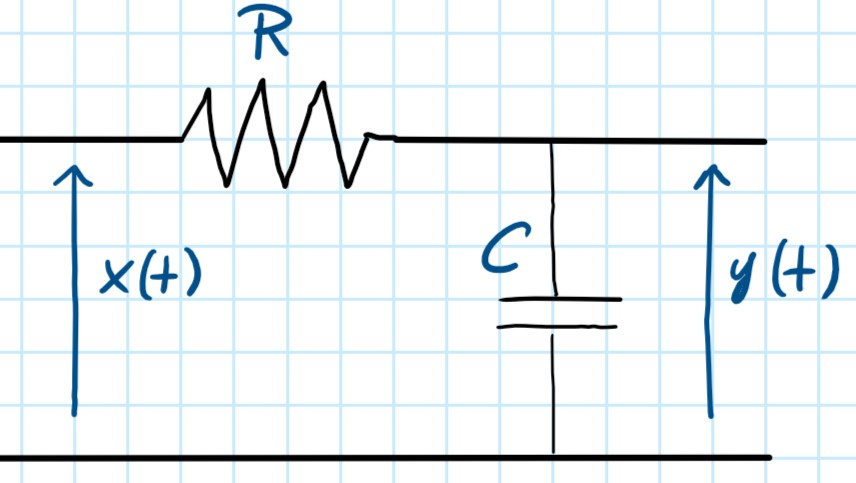
\includegraphics[width=5cm]{passivelowpass}
			\caption{schematic representation of the "common" passive low-pass filter.}
			\label{fig:ex:lowpass}
		\end{SCfigure}
		
		Considering the passive low-pass filer in figure \ref{fig:ex:lowpass} where $x(t)$ is the input voltage and $y(t)$ the output voltage, given $i(t)$ the current passing through the resistor then from the Kirchhoff laws we have to impose the relation
		\[ x(t) = Ri(t) + y(t) \]
		Considering that the current $i(t)$ depends from the voltage difference between the capacitor following the differential equation $i(t) = C\dot y(t)$ then the differential equation solution of the transient is
		\[ x(t) = RC \dot y(t) + y(t) \]
		The solution can be obtained in the frequency domain: applying the \ctft we determine an algebraic equation that can solve the spectrum of the output:
		\[ X(j\Omega) = j\Omega RC Y(j\Omega) + Y(j\Omega) \qquad \Rightarrow \qquad Y(j\Omega) = \frac 1{1 + j\Omega RC} X(j\Omega)\]
		where we can recognize the well-known frequency response $H(j\Omega) = \frac 1{1 + j\Omega RC}$ of the low pass filter that by inversion determines the impulse response
		\[ h(t) = \frac 1{RC} e^{-\frac{t}{RC}} u(t) \hspace{2cm} u(t) = \begin{cases}
			1 & t\geq 0 \\ 0 & t < 0
		\end{cases} \]
		\begin{note}
			when the Fourier transform was applied on the differential equation as initial condition a value $y(0)= 0$ has been set.
		\end{note}
		\begin{SCfigure}[2][bht]
			\centering \includegraphics[width=4.5cm]{ex-lowpass-1}
			\caption{impulse response of the low pass filter considering a value $RC=2$.}
		\end{SCfigure}
		
		\paragraph{Response to a rectangular input} Considering now the case of a rectangular input signal of amplitude $A$ and duration $T$ starting from $t=0$ (as was in figure \ref{fig:ex:signals}.a), the definition of the output is more complex due to the fact that the low-pass filter present an infinite impulse response (respect to the finite impulse response of the example in figure \ref{fig:ex:signals}.b). Computing the output of the system as the convolution
		\[ y(t) = h(t)*x(t) \]
		considering $h (\tau)$ as the \textit{fixed} signal, the flipped signal $x(-\tau)$ is instead \textit{moved} along the horizontal axis. Until $t<0$ the moving rectangle doesn't overlap with the exponential response, thus $y(t) = 0$; for $0\leq t\leq T$ we have the continuous insertion of the rectangle and by computing the integral we obtain
		\[ y(t) = \int_0^t \frac 1{RC}e^{-\frac{\tau}{RC}}\cdot A\, d\tau = A\left( 1-e^{-\frac{t}{RC}} \right) \]
		For $t>T$, due to the infinite impulse response, the convolution gives the output
		\[ y(t) = \int_{t-T}^t \frac 1{RC}e^{-\frac{\tau}{RC}}\cdot A\, d\tau = A\left( e^{-\frac{tT}{RC}} - e^{-\frac{t}{RC}} \right) \]
		The complete output of the system is so
		\[ y(t) = \begin{cases}
			0 \qquad & t < 0 \\
			A \big( 1-e^{-\frac{t}{RC}} \big) & 0 \leq t \leq T \\
			A \big( e^{-\frac{tT}{RC}} - e^{-\frac{t}{RC}}  \big) \quad & t>T
		\end{cases}\]
		\begin{SCfigure}[2][bht]
			\centering \includegraphics[width=4.5cm]{ex-lowpass-2}
			\caption{output voltage $y(t)$ of a low pass filter subjected to a rectangular pulse of amplitude $A=1$, duration $T=3$ and starting at $t=0$ considering a value $RC=2$.}
		\end{SCfigure}
		
		\paragraph{Finite difference} While dealing with numerical methods determining analytical result (as previously done) is impossible and a discrete-time formulation of the problem must be presented. Considering a discretized problem where the time is sampled with a constant period $T_s$ the current $i(t)$ flowing through the resistor can be approximated by the \textbf{backward Euler difference} for derivation as
		\begin{equation}
			i(nT_s) = C \left.\frac{dy}{dt}\right|_{t=nT_s} \approx C \frac{y\big(nT_s\big) - y\big((n-1)T_s\big) }{T_s}
		\end{equation}
		With this definition we can rewrite the \textbf{discrete-time equivalent model} of the low pass filter as
		\[ x(nT_s) = RC \frac{y\big(nT_s\big) - y\big((n-1)T_s\big) }{T_s} + y(nT_s) \]
		Considering the full discrete equivalence ($x(n) = x(nT_s)$ and $y(n) = y(nT_s)$) the previous equation can be manipulated in order to express the output $y(n)$ as function of the previous outputs $y(n-1)$ and current input $x(n)$:
		\begin{align*}
			y(n) - y(n-1) + \frac{T_s}{RC} y(n) & = \frac{T_s}{RC} x(n) \\
			\left(1 + \frac{T_s}{RC}\right) y(n) & = \frac{T_s}{RC} x(n) + y(n-1)\\
			y(n) & = a y(n-1) + (1-a) x(n)
		\end{align*}
		where $a = \frac{1}{1+ \frac{T_s}{RC}}$; considering the term $b = 1-a = \frac{T_s}{RC + T_s}$, the impulse response of the discrete-time equivalent system is generated by imposing that $y(-1) = 0$ and $x(n) = \delta(n)$ (all inputs are pulses) and so we have
		\[ \begin{cases}
			n = 0 \qquad  & \rightarrow \quad y(0) = h(0) = 1- a = b\\
			n = 1 \qquad  & \rightarrow \quad y(1) = h(1) = (1-a)a = ba\\
			n = 2 \qquad  & \rightarrow \quad y(2) = h(2) = (1-a)a^2 = ba^2\\
			& \hspace{4pt} \vdots \\
			n = k \qquad  & \rightarrow \quad y(k) = h(k) = (1-a)a^k = ba^k \\
		\end{cases} \]
		and so the general formulation is
		\begin{equation}
			h(n) = b a^n \, u(n) \hspace{2cm} \textrm{where } u(n) = \begin{cases}
				1 & n\geq 0 \\ 0 & n < 0
			\end{cases}
		\end{equation}
		
		
		
		
		
		
		
		
		